\documentclass{standalone}
\usepackage{tikz}
\usetikzlibrary{patterns, positioning}

\begin{document}
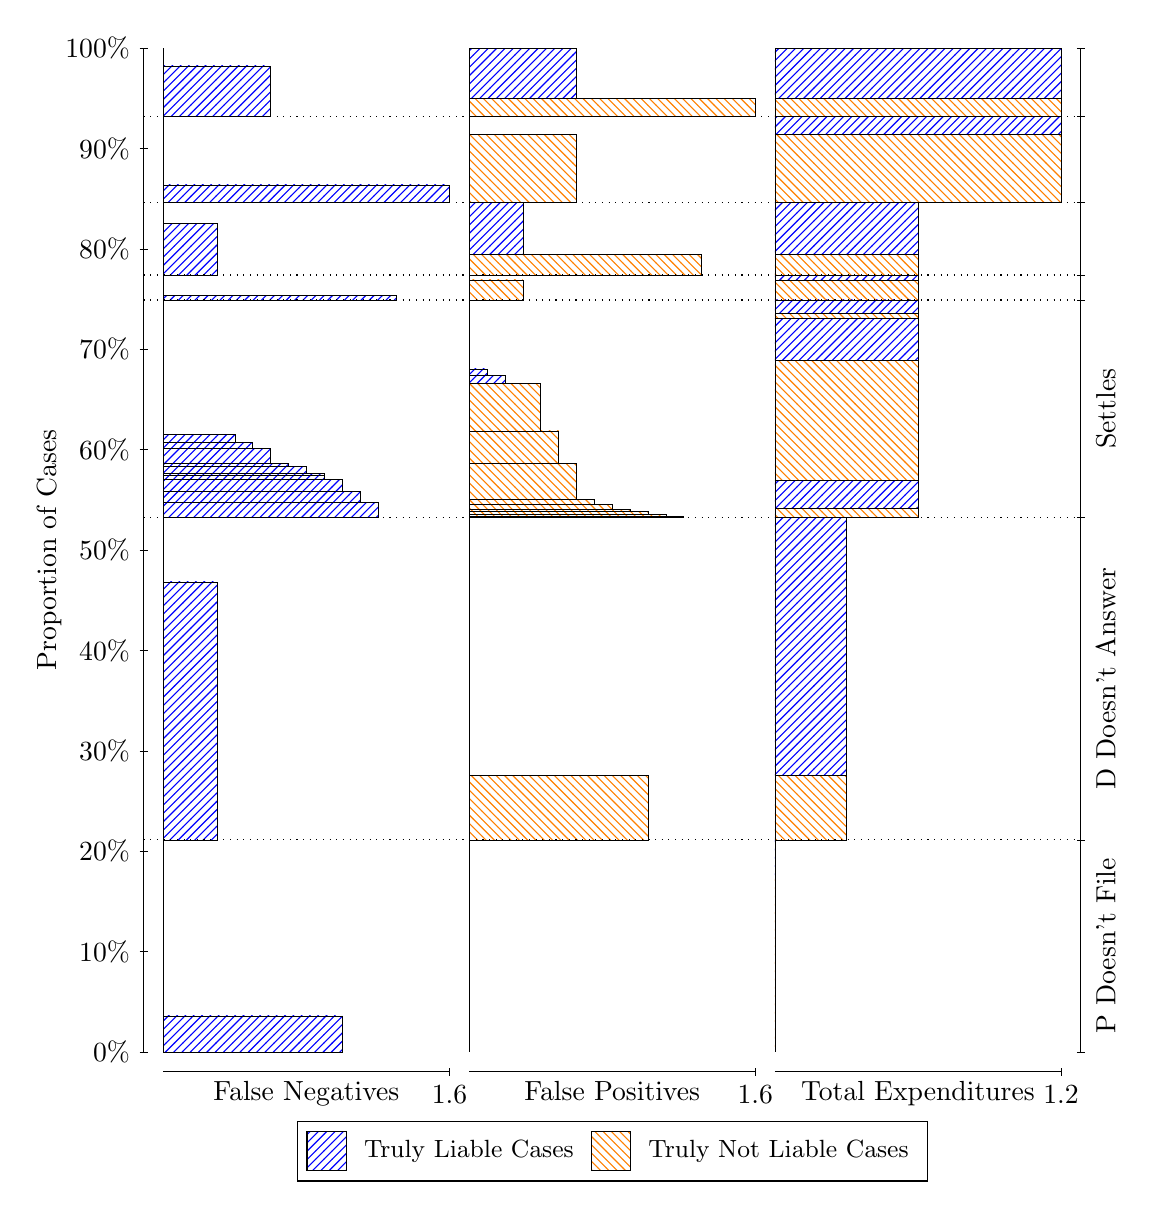
\begin{tikzpicture}
\draw[black, very thin] (1.5,1.75) -- (1.5,14.5);
\node[rotate=90, anchor=center] at (0.3, 8.125) {Proportion of Cases};
\draw[black, very thin] (1.45,1.75) -- (1.55,1.75);
\node[anchor=east] at (1.45, 1.75) {0\%};
\draw[black, very thin] (1.45,3.025) -- (1.55,3.025);
\node[anchor=east] at (1.45, 3.025) {10\%};
\draw[black, very thin] (1.45,4.3) -- (1.55,4.3);
\node[anchor=east] at (1.45, 4.3) {20\%};
\draw[black, very thin] (1.45,5.575) -- (1.55,5.575);
\node[anchor=east] at (1.45, 5.575) {30\%};
\draw[black, very thin] (1.45,6.85) -- (1.55,6.85);
\node[anchor=east] at (1.45, 6.85) {40\%};
\draw[black, very thin] (1.45,8.125) -- (1.55,8.125);
\node[anchor=east] at (1.45, 8.125) {50\%};
\draw[black, very thin] (1.45,9.4) -- (1.55,9.4);
\node[anchor=east] at (1.45, 9.4) {60\%};
\draw[black, very thin] (1.45,10.675) -- (1.55,10.675);
\node[anchor=east] at (1.45, 10.675) {70\%};
\draw[black, very thin] (1.45,11.95) -- (1.55,11.95);
\node[anchor=east] at (1.45, 11.95) {80\%};
\draw[black, very thin] (1.45,13.225) -- (1.55,13.225);
\node[anchor=east] at (1.45, 13.225) {90\%};
\draw[black, very thin] (1.45,14.5) -- (1.55,14.5);
\node[anchor=east] at (1.45, 14.5) {100\%};

\draw[black, very thin] (13.4,1.75) -- (13.4,14.5);
\draw[black, very thin] (13.35,1.75) -- (13.45,1.75);
\node[anchor=west] at (13.35, 1.75) {};
\draw[black, very thin] (13.35,4.4428) -- (13.45,4.4428);
\node[anchor=west] at (13.35, 4.4428) {};
\draw[black, very thin] (13.35,8.5383) -- (13.45,8.5383);
\node[anchor=west] at (13.35, 8.5383) {};
\draw[black, very thin] (13.35,11.3) -- (13.45,11.3);
\node[anchor=west] at (13.35, 11.3) {};
\draw[black, very thin] (13.35,11.617) -- (13.45,11.617);
\node[anchor=west] at (13.35, 11.617) {};
\draw[black, very thin] (13.35,12.535) -- (13.45,12.535);
\node[anchor=west] at (13.35, 12.535) {};
\draw[black, very thin] (13.35,13.63) -- (13.45,13.63);
\node[anchor=west] at (13.35, 13.63) {};
\draw[black, very thin] (13.35,14.5) -- (13.45,14.5);
\node[anchor=west] at (13.35, 14.5) {};

\draw[black, very thin, pattern color=blue, pattern=north east lines] (1.75,1.75) rectangle (4.0208,2.2072);
\draw[black, very thin, pattern color=orange, pattern=north west lines] (1.75,2.2072) rectangle (1.75,4.4428);
\draw[black, very thin, pattern color=blue, pattern=north east lines] (1.75,4.4428) rectangle (2.4312,7.7199);
\draw[black, very thin, pattern color=orange, pattern=north west lines] (1.75,7.7199) rectangle (1.75,8.5383);
\draw[black, very thin, pattern color=blue, pattern=north east lines] (1.75,8.5383) rectangle (4.475,8.7308);
\draw[black, very thin, pattern color=blue, pattern=north east lines] (1.75,8.7308) rectangle (4.2479,8.8661);
\draw[black, very thin, pattern color=blue, pattern=north east lines] (1.75,8.8661) rectangle (4.0208,9.0184);
\draw[black, very thin, pattern color=blue, pattern=north east lines] (1.75,9.0184) rectangle (3.7937,9.0753);
\draw[black, very thin, pattern color=blue, pattern=north east lines] (1.75,9.0753) rectangle (3.7937,9.1011);
\draw[black, very thin, pattern color=blue, pattern=north east lines] (1.75,9.1011) rectangle (3.5667,9.1871);
\draw[black, very thin, pattern color=blue, pattern=north east lines] (1.75,9.1871) rectangle (3.3396,9.229);
\draw[black, very thin, pattern color=blue, pattern=north east lines] (1.75,9.229) rectangle (3.1125,9.4124);
\draw[black, very thin, pattern color=blue, pattern=north east lines] (1.75,9.4124) rectangle (2.8854,9.4962);
\draw[black, very thin, pattern color=blue, pattern=north east lines] (1.75,9.4962) rectangle (2.6583,9.594);
\draw[black, very thin, pattern color=orange, pattern=north west lines] (1.75,9.594) rectangle (1.75,11.3);
\draw[black, very thin, pattern color=blue, pattern=north east lines] (1.75,11.3) rectangle (4.7021,11.361);
\draw[black, very thin, pattern color=orange, pattern=north west lines] (1.75,11.361) rectangle (1.75,11.617);
\draw[black, very thin, pattern color=blue, pattern=north east lines] (1.75,11.617) rectangle (2.4312,12.27);
\draw[black, very thin, pattern color=orange, pattern=north west lines] (1.75,12.27) rectangle (1.75,12.535);
\draw[black, very thin, pattern color=blue, pattern=north east lines] (1.75,12.535) rectangle (5.3833,12.763);
\draw[black, very thin, pattern color=orange, pattern=north west lines] (1.75,12.763) rectangle (1.75,13.63);
\draw[black, very thin, pattern color=blue, pattern=north east lines] (1.75,13.63) rectangle (3.1125,14.273);
\draw[black, very thin, pattern color=orange, pattern=north west lines] (1.75,14.273) rectangle (1.75,14.5);
\draw[black, very thin, pattern color=orange, pattern=north west lines] (5.6333,1.75) rectangle (5.6333,3.9856);
\draw[black, very thin, pattern color=blue, pattern=north east lines] (5.6333,3.9856) rectangle (5.6333,4.4428);
\draw[black, very thin, pattern color=orange, pattern=north west lines] (5.6333,4.4428) rectangle (7.9042,5.2612);
\draw[black, very thin, pattern color=blue, pattern=north east lines] (5.6333,5.2612) rectangle (5.6333,8.5383);
\draw[black, very thin, pattern color=orange, pattern=north west lines] (5.6333,8.5383) rectangle (8.3583,8.5558);
\draw[black, very thin, pattern color=orange, pattern=north west lines] (5.6333,8.5558) rectangle (8.1313,8.5729);
\draw[black, very thin, pattern color=orange, pattern=north west lines] (5.6333,8.5729) rectangle (7.9042,8.611);
\draw[black, very thin, pattern color=orange, pattern=north west lines] (5.6333,8.611) rectangle (7.6771,8.6375);
\draw[black, very thin, pattern color=orange, pattern=north west lines] (5.6333,8.6375) rectangle (7.45,8.703);
\draw[black, very thin, pattern color=orange, pattern=north west lines] (5.6333,8.703) rectangle (7.2229,8.7682);
\draw[black, very thin, pattern color=orange, pattern=north west lines] (5.6333,8.7682) rectangle (6.9958,9.2263);
\draw[black, very thin, pattern color=orange, pattern=north west lines] (5.6333,9.2263) rectangle (6.7687,9.6378);
\draw[black, very thin, pattern color=orange, pattern=north west lines] (5.6333,9.6378) rectangle (6.5417,10.244);
\draw[black, very thin, pattern color=blue, pattern=north east lines] (5.6333,10.244) rectangle (6.0875,10.342);
\draw[black, very thin, pattern color=blue, pattern=north east lines] (5.6333,10.342) rectangle (5.8604,10.426);
\draw[black, very thin, pattern color=blue, pattern=north east lines] (5.6333,10.426) rectangle (5.6333,11.3);
\draw[black, very thin, pattern color=orange, pattern=north west lines] (5.6333,11.3) rectangle (6.3146,11.556);
\draw[black, very thin, pattern color=blue, pattern=north east lines] (5.6333,11.556) rectangle (5.6333,11.617);
\draw[black, very thin, pattern color=orange, pattern=north west lines] (5.6333,11.617) rectangle (8.5854,11.882);
\draw[black, very thin, pattern color=blue, pattern=north east lines] (5.6333,11.882) rectangle (6.3146,12.535);
\draw[black, very thin, pattern color=orange, pattern=north west lines] (5.6333,12.535) rectangle (6.9958,13.402);
\draw[black, very thin, pattern color=blue, pattern=north east lines] (5.6333,13.402) rectangle (5.6333,13.63);
\draw[black, very thin, pattern color=orange, pattern=north west lines] (5.6333,13.63) rectangle (9.2667,13.857);
\draw[black, very thin, pattern color=blue, pattern=north east lines] (5.6333,13.857) rectangle (6.9958,14.5);
\draw[black, very thin, pattern color=orange, pattern=north west lines] (9.5167,1.75) rectangle (9.5167,3.9856);
\draw[black, very thin, pattern color=blue, pattern=north east lines] (9.5167,3.9856) rectangle (9.5167,4.4428);
\draw[black, very thin, pattern color=orange, pattern=north west lines] (9.5167,4.4428) rectangle (10.425,5.2612);
\draw[black, very thin, pattern color=blue, pattern=north east lines] (9.5167,5.2612) rectangle (10.425,8.5383);
\draw[black, very thin, pattern color=orange, pattern=north west lines] (9.5167,8.5383) rectangle (11.333,8.6591);
\draw[black, very thin, pattern color=blue, pattern=north east lines] (9.5167,8.6591) rectangle (11.333,9.0123);
\draw[black, very thin, pattern color=orange, pattern=north west lines] (9.5167,9.0123) rectangle (11.333,10.532);
\draw[black, very thin, pattern color=blue, pattern=north east lines] (9.5167,10.532) rectangle (11.333,11.069);
\draw[black, very thin, pattern color=orange, pattern=north west lines] (9.5167,11.069) rectangle (11.333,11.134);
\draw[black, very thin, pattern color=blue, pattern=north east lines] (9.5167,11.134) rectangle (11.333,11.3);
\draw[black, very thin, pattern color=orange, pattern=north west lines] (9.5167,11.3) rectangle (11.333,11.556);
\draw[black, very thin, pattern color=blue, pattern=north east lines] (9.5167,11.556) rectangle (11.333,11.617);
\draw[black, very thin, pattern color=orange, pattern=north west lines] (9.5167,11.617) rectangle (11.333,11.882);
\draw[black, very thin, pattern color=blue, pattern=north east lines] (9.5167,11.882) rectangle (11.333,12.535);
\draw[black, very thin, pattern color=orange, pattern=north west lines] (9.5167,12.535) rectangle (13.15,13.402);
\draw[black, very thin, pattern color=blue, pattern=north east lines] (9.5167,13.402) rectangle (13.15,13.63);
\draw[black, very thin, pattern color=orange, pattern=north west lines] (9.5167,13.63) rectangle (13.15,13.857);
\draw[black, very thin, pattern color=blue, pattern=north east lines] (9.5167,13.857) rectangle (13.15,14.5);
\draw[black, dotted] (1.5,4.4428) -- (13.4,4.4428);
\draw[black, dotted] (1.5,8.5383) -- (13.4,8.5383);
\draw[black, dotted] (1.5,11.3) -- (13.4,11.3);
\draw[black, dotted] (1.5,11.617) -- (13.4,11.617);
\draw[black, dotted] (1.5,12.535) -- (13.4,12.535);
\draw[black, dotted] (1.5,13.63) -- (13.4,13.63);
\draw[black, very thin] (1.75,1.5) -- (5.3833,1.5);
\node[anchor=north] at (3.5667, 1.5) {False Negatives};
\draw[black, very thin] (5.3833,1.45) -- (5.3833,1.55);
\node[anchor=north] at (5.3833, 1.45) {1.6};

\draw[black, very thin] (5.6333,1.5) -- (9.2667,1.5);
\node[anchor=north] at (7.45, 1.5) {False Positives};
\draw[black, very thin] (9.2667,1.45) -- (9.2667,1.55);
\node[anchor=north] at (9.2667, 1.45) {1.6};

\draw[black, very thin] (9.5167,1.5) -- (13.15,1.5);
\node[anchor=north] at (11.333, 1.5) {Total Expenditures};
\draw[black, very thin] (13.15,1.45) -- (13.15,1.55);
\node[anchor=north] at (13.15, 1.45) {1.2};

\node[black, centered, rotate=90] at (13.72, 3.0964) {P Doesn't File};
\node[black, centered, rotate=90] at (13.72, 6.4906) {D Doesn't Answer};
\node[black, centered, rotate=90] at (13.72, 9.919) {Settles};





\draw (7.449999999999999,1.5) node[draw=none] (baseCoordinate) {};
\begin{scope}[align=center]
        \matrix[scale=0.5, draw=black, below=0.5cm of baseCoordinate, nodes={draw}, column sep=0.1cm]{
            \node[rectangle, draw, minimum width=0.5cm, minimum height=0.5cm, pattern=north east lines, pattern color=blue] {}; &
            \node[draw=none, font=\small] (B) {Truly Liable Cases}; &
            \node[rectangle, draw, minimum width=0.5cm, minimum height=0.5cm, pattern=north west lines, pattern color=orange] {}; &
            \node[draw=none, font=\small] (B) {Truly Not Liable Cases}; \\
            };
\end{scope}

\end{tikzpicture}
\end{document}